\section*{ANALYSIS}\label{analysis}
\hypertarget{fnpf}{%
\subsection*{FNPF}\label{fnpf}}
The FNPF results have the benifit of having all the three states:
$\phi$, $\dot{\phi}$ and $\ddot{\phi}$. This means that these time
series can be inserted into the differential equation
(Eq.\ref{eq:eqroll_decay_equation_quadratic_a}) and the
parameters of the model can be estimated using Ordinary Least Square
method (OLS), solving the following regression:
\begin{equation}
y = X \cdot \beta + \epsilon
\label{ols}
\end{equation}
where:
\begin{itemize}
\item $y$ is the dependent variable (also called *label*).
\item $\beta$ is a vector with the regressed parameters.
\item $X$ is a matrix containing the independent variables (also called *features*).
\end{itemize}
The roll decay equation can be expressed as a linear regression with
\begin{itemize}
\item $y$ : the roll angle acceleration $\ddot{\phi}$
\item $\beta$ : contains all the parameters : $B_1$, $B_2$, $C_1$...
\item $X$ : contains all the time varying features such as: $| \dot{\phi} | \dot{\phi} $ etc.
\end{itemize}
So the roll acceleration is put on the left hand side:
\begin{equation}
\begin{aligned}
- \ddot{\phi} = B_{1A} \dot{\phi} + B_{2A} \left|{\dot{\phi}}\right| \dot{\phi} + B_{3A} \dot{\phi}^{3} + C_{1A} \phi + C_{3A} \phi^{3} \\ + C_{5A} \phi^{5}
\end{aligned}
\label{acceleration_equation_cubic}
\end{equation}
The equation for the acceleration
Eq.\ref{eq:acceleration_equation_cubic} can now be rewritten as
the linear regression in Eq.\ref{eq:ols}, where:
$\displaystyle \beta = \left[\begin{matrix}B_{1A}\\B_{2A}\\B_{3A}\\C_{1A}\\C_{3A}\\C_{5A}\end{matrix}\right]$
\begin{equation}
X = \left[\begin{matrix}\dot{\phi} & \left|{\dot{\phi}}\right| \dot{\phi} & \dot{\phi}^{3} & \phi & \phi^{3} & \phi^{5}\end{matrix}\right]
\label{eq_X}
\end{equation}
\begin{equation}
y = - \ddot{\phi}
\label{eq_y}
\end{equation}
The coefficients determined with Ordinary Least Square fit is shown in
Tab.\ref{tab:parameters}. The mean value of these coefficients
are presented togehter with 5\% confidence level intervalls.
\begin{table}[H]
\scriptsize
\center
\caption{Parameters estimation cubic model}
\label{tab:parameters}
\begin{tabular}{|l|l|l|l|l|}
\hline\addlinespace
coeff & mean & P>|t| & $conf_{lower}$ & $conf_{higher}$\\
B_1A & 0.016 & 0.0 & 0.014 & 0.018\\
\hlineB_2A & -0.062 & 0.0 & -0.076 & -0.047\\
B_3A & 0.098 & 0.0 & 0.072 & 0.124\\
C_1A & 6.116 & 0.0 & 6.114 & 6.118\\
C_3A & -5.522 & 0.0 & -5.807 & -5.236\\
C_5A & 254.093 & 0.0 & 244.923 & 263.264\\
\hline
\end{tabular}
\end{table}
\hypertarget{simulation}{%
\subsection*{Simulation}\label{simulation}}
Fig.\ref{fig:sim_cubic} shows a simulation with the regressed
parameters together with the original data from the FNPF simulations.
\begin{figure}[H]
\begin{center}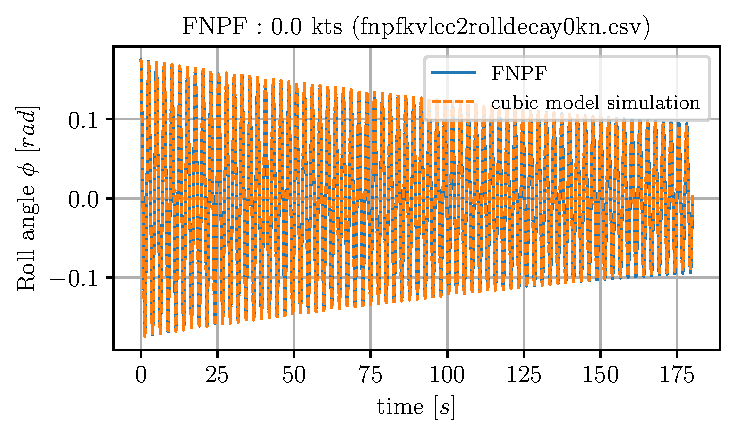
\includegraphics[width = 0.95\textwidth]{figures/sim_cubic.pdf}\end{center}
\vspace{-0.7cm}
\caption{Simulation of roll decay test with parameters from the cubic model.}
\label{fig:sim_cubic}
\end{figure}
\begin{equation}
- \ddot{\phi} = B_{1A} \dot{\phi} + C_{1A} \phi
\label{Eq(-Derivative(phi(t), (t, 2)), B_1A*Derivative(phi(t), t) + C_1A*phi(t))}
\end{equation}
\begin{equation}
X_{2} = \left[\begin{matrix}\dot{\phi} & \phi\end{matrix}\right]
\label{eq_X2}
\end{equation}\displaystyle \beta_{2} = \left[\begin{matrix}B_{1A}\\C_{1A}\end{matrix}\right]$
\begin{table}[H]
\scriptsize
\center
\caption{Parameters estimation linear model}
\label{tab:parameters}
\begin{tabular}{|l|l|l|l|l|}
\hline\addlinespace
coeff & mean & P>|t| & $conf_{lower}$ & $conf_{higher}$\\
B_1A & 0.007 & 0.0 & 0.007 & 0.007\\
\hlineC_1A & 6.101 & 0.0 & 6.1 & 6.101\\
\hline
\end{tabular}
\end{table}
\begin{figure}[H]
\begin{center}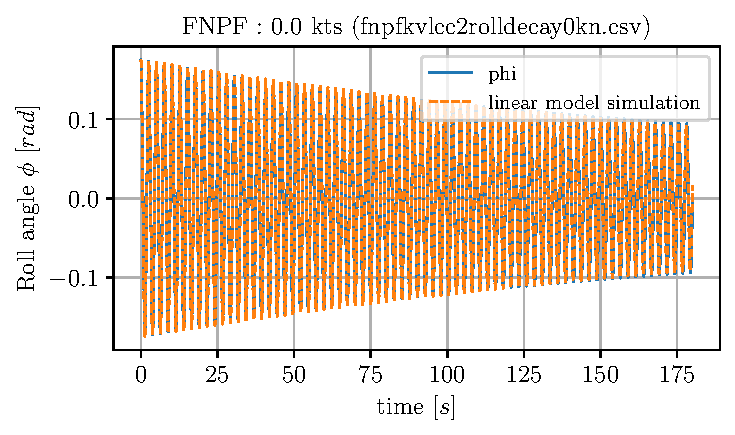
\includegraphics[width = 0.95\textwidth]{figures/sim_linear.pdf}\end{center}
\vspace{-0.7cm}
\caption{Simulation of roll decay test with parameters from the linear model.}
\label{fig:sim_linear}
\end{figure}
The coefficient of determination $R^2$ is very similar between the
cubic (0.997) and the linear model (0.989), when comparing simulated
roll signal with the corresponding data from FNPF.
